\documentclass[11pt,letterpaper]{article}

\usepackage{graphicx}
\usepackage{mathpazo}

\usepackage{minted}
\usemintedstyle{arduino}

\usepackage{geometry}
\geometry{margin=1in}

\title{Triangle/Spumpus Plot GNUPlot Output and Code}
\author{Alex Striff}
\date{August 26, 2018}

\begin{document}
\maketitle

\begin{figure}[H]
  \centering
  \colorbox{white}{%
    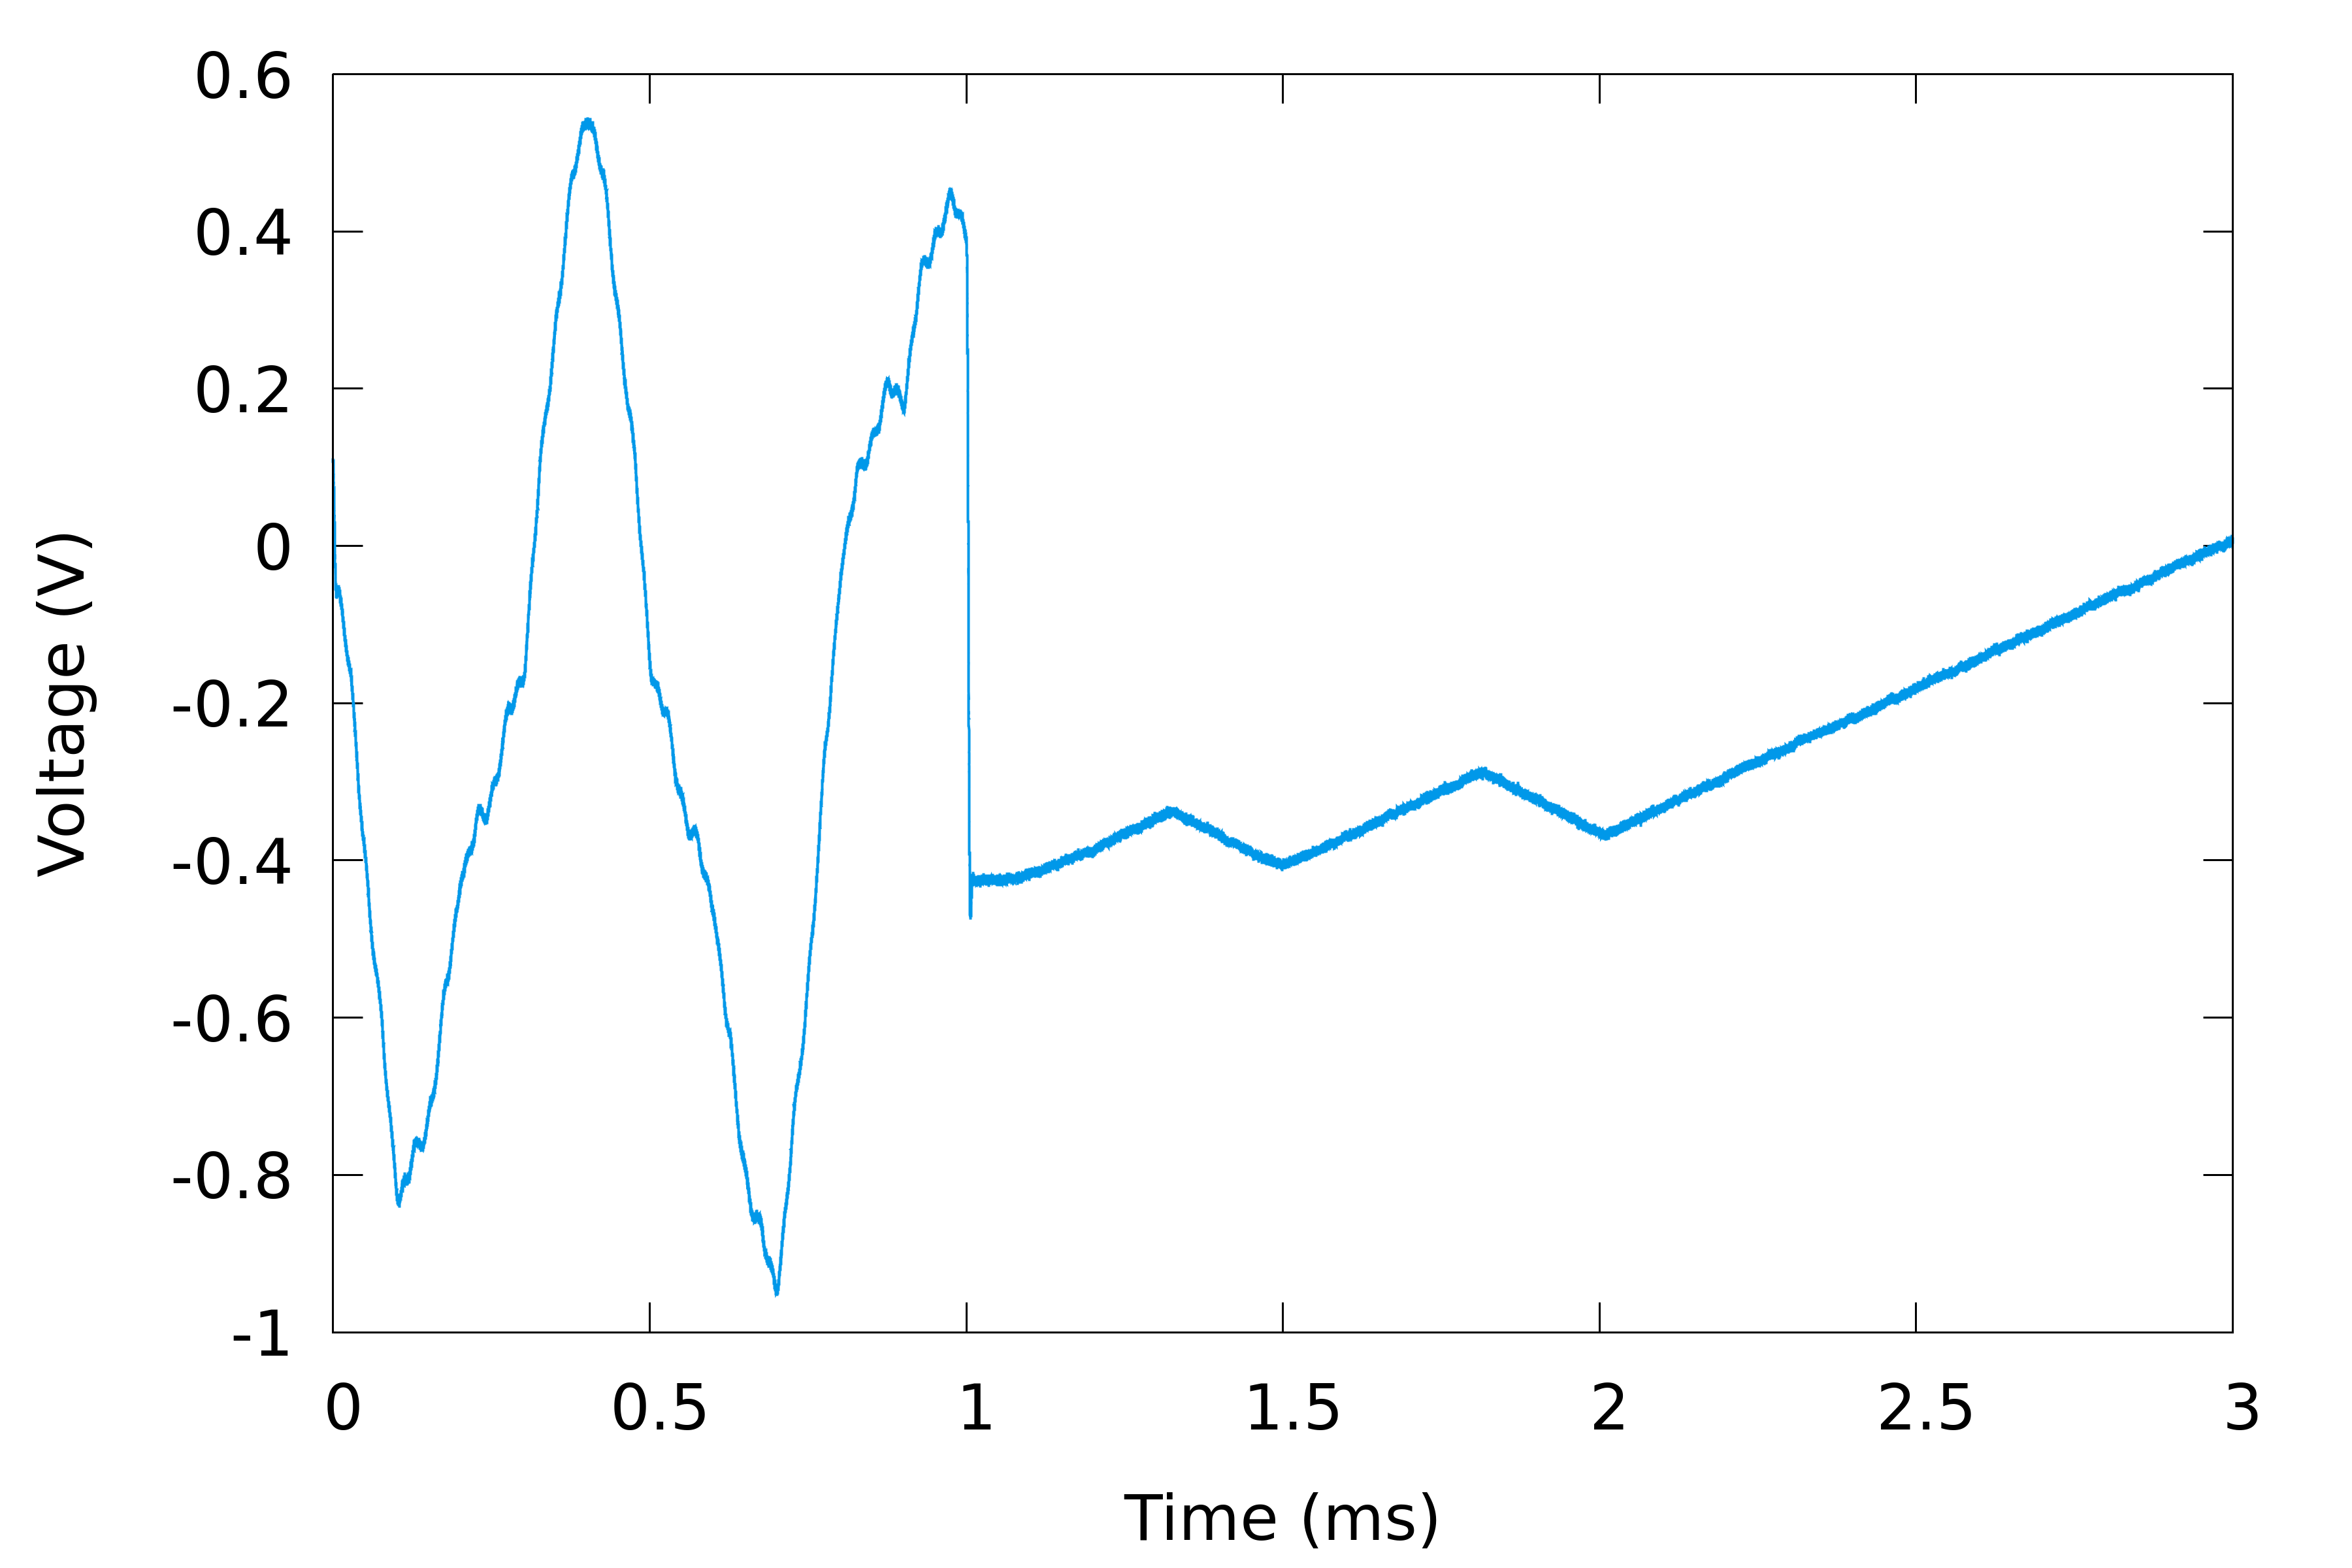
\includegraphics[width=\linewidth]{../spumpus-pc.png}
  }
  \caption{Paper, color version.}
\end{figure}
\begin{figure}[H]
  \centering
  \colorbox{white}{%
    
\includegraphics[width=\linewidth]{../spumpus-pg.png}
  }
  \caption{Paper, grayscale version.}
\end{figure}
\begin{figure}[H]
  \centering
  \colorbox{black}{%
    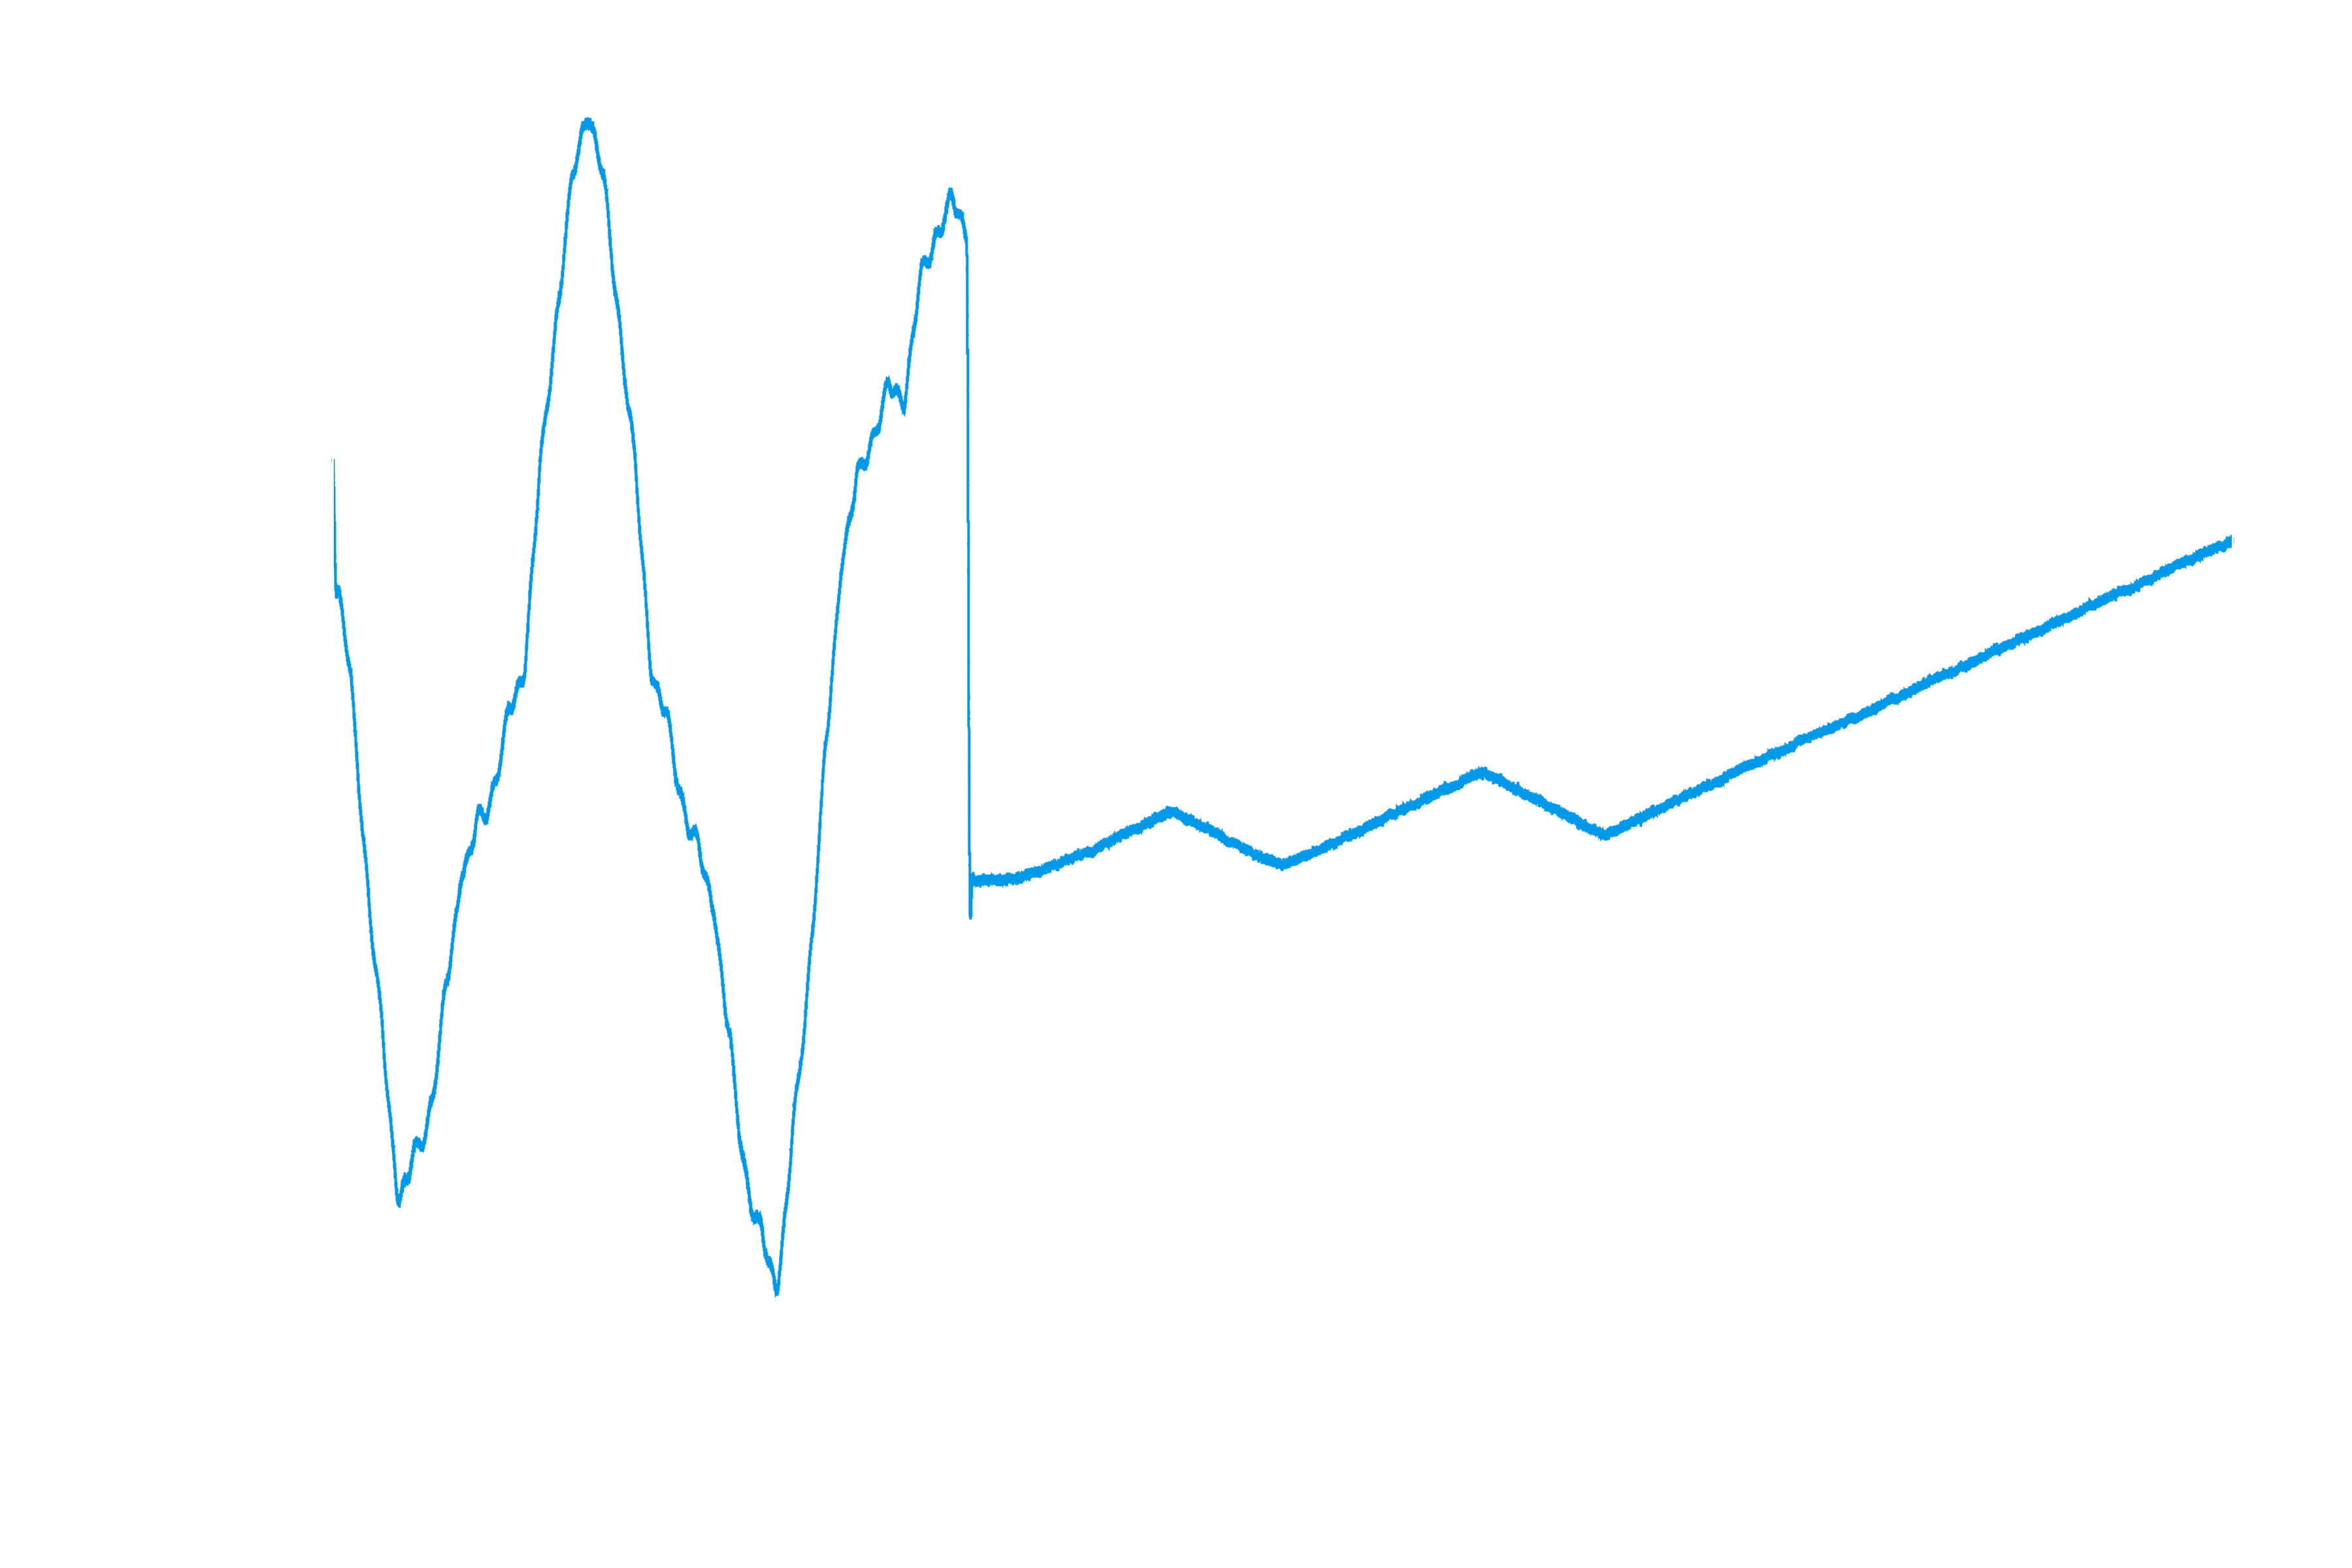
\includegraphics[width=\linewidth]{../spumpus-do.png}
  }
  \caption{Dark Owl version (beamer slides).}
\end{figure}

\begin{minted}{gnuplot}
set terminal pngcairo transparent enhanced font "Droid Sans,72" \
      fontscale 1.0 size 3600, 2400

# Dark Owl
text = '#ffffff'
spcolor = '#0098e9' # OwlBlue
set output 'spumpus-do.png'

# Paper Color
# text = '#000000'
# spcolor = '#0098e9' # OwlBlue
# set output 'spumpus-pc.png'

# Paper Grayscale
# text = '#000000'
# spcolor = '#000000'
# set output 'spumpus-pg.png'

set style increment default

set border lw 3 lc rgb text
set xlabel tc rgb text
set ylabel tc rgb text

set datafile separator ','
sphist = 'spumpus-hist.csv'
spout  = 'spumpus-out.csv'

unset key
set xlabel 'Time (ms)'
set ylabel 'Voltage (V)'
set xrange [0:3] noreverse writeback

plot \
       sphist u ($1 * 1e3):($2) w lines lw 4 lt rgb spcolor

\end{minted}

\end{document}


